\section{Swaps}\label{sec:swaps}


Los \textbf{swaps} son contratos en los que dos partes acuerdan intercambiar flujos de efectivo futuro según una fórmula preestablecida. En un primer momento lo típico eran swaps de divisas, pero derivó en swaps de intereses.



\subsection{Swaps de intereses vainillas}
Contratos bastante comunes en los que se intercambian flujos de intereses. Por ejemplo, una parte paga un tipo fijo y la otra un tipo variable como el Euribor a 3 meses, 6 meses, etc. A vencimiento, los principales no se intercambian, solo los intereses.
\begin{figure}[H]
    \centering
    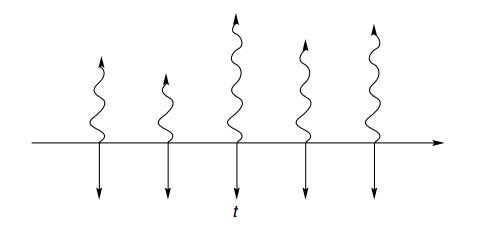
\includegraphics[width=0.65\linewidth]{Imagenes/Parte1/12_swaps/Interest_swap.png}
    \caption{Swaps de intereses vainillas}
\end{figure}
\subsubsection{Ejemplo de uso}
Dos empresas, A y B quieren pedir un préstamo, A quiere que sea variable y B que sea fijo. Los intereses que les cobran estan en la siguiente tabla:
\begin{table}[H]
    \centering
    \begin{tabular}[H]{|l|c|c|}
        \hline
        & \textbf{Fijo} & \textbf{Variable} \\
        \hline
        \textbf{A} & 7\% & \text{LIBOR a 6 meses} + 0.3\% \\
        \hline
        \textbf{B} & 8.2\% & \text{LIBOR a 6 meses} + 1\% \\
        \hline
    \end{tabular}
\end{table}
Luego si ambos piden el préstamos los intereses que pagan son:
\begin{itemize}
    \item A variable y B fijo:
    \[
        \text{LIBOR} + 0.3\% + 8.2\% = \text{LIBOR} + 8.5\%
    \]
    \item A fijo y B variable:
    \[
        7\% + \text{LIBOR} + 1\% = \text{LIBOR} + 8\%
    \]
\end{itemize}
Luego es mejor la segunda opción, pero como no es el tipo de interés que quieren cada uno, hacen un swap. Se reparten los inetreses extra de manera equitativa. Para dar la vuelta al tipo de interés, en el swap A le paga a B el LIBOR y B le paga una cantidad fija $x$\%. Entonces:
\begin{align*}
    \text{A: } & \underbrace{7\%}_{\text{int A fijo}} + \underbrace{\text{LIBOR}}_{\text{pago swap}} - \underbrace{x\% }_{\text{cobro swap}} + \underbrace{\frac{0.5}{2}\%}_{\text{int extra}} =  \underbrace{\text{LIBOR} + 0.3\%}_{\text{int A variable}} \Rightarrow x = 6.95\%\\
    \text{B: } & \underbrace{\text{LIBOR} + 1\%}_{\text{int B variable}} + \underbrace{x\%}_{\text{pago swap}} - \underbrace{\text{LIBOR}}_{\text{cobro swap}} + \underbrace{\frac{0.5}{2}\%}_{\text{int extra}} =  \underbrace{8.2\%}_{\text{int B fijo}} \Rightarrow x = 6.95\%
\end{align*}
por lo tanto, las empresas A y B pagan un interés:
\begin{align*}
    \text{A: } & \underbrace{7\%}_{\text{int A fijo}} + \underbrace{\text{LIBOR}}_{\text{pago swap}} - \underbrace{6.95\% }_{\text{cobro swap}} =  \text{LIBOR} + 0.05\% \\
    \text{B: } & \underbrace{\text{LIBOR} + 1\%}_{\text{int B variable}} + \underbrace{6.95\%}_{\text{pago swap}} - \underbrace{\text{LIBOR}}_{\text{cobro swap}} =  7.95\%
\end{align*}
que es tipo de interés que quería cada empresa y es mejor que si hubieran pedido el préstamo directamente con los intereses de la tabla.









\subsection{Relación entre swaps y bonos: obtener valor justo del interés fijo}
En primer lugar, el interés fijo se puede ver como un bono de cupón cero. Por lo tanto, el total de pagos por parte del interés fijo es
\[
    r_s\tau \sum_{i=1}^N Z(t;T_i)
\]
donde $r_s$ es el interés (p.e.\ anual), $\tau$ es el tiempo entre pagos (escrito en la misma escala que el interés, p.e.\ 0.5 años) y $Z(t;T)$ es el valor actualizado de un bono de cupón cero y principal 1.

Por otro lado, se debe escribir el valor de los intereses variables pagados en términos de un bono. Se tiene el siguiente esquema para el pago del interés variable en tiempo $T_i$:
 \begin{figure}[H]
    \centering
    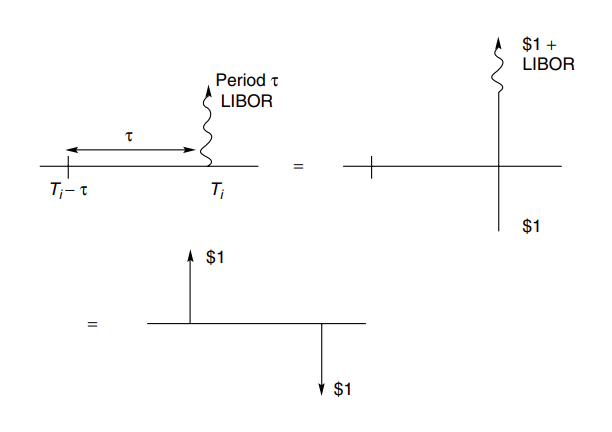
\includegraphics[width=0.65\linewidth]{Imagenes/Parte1/12_swaps/Relacion_Swaps_Bonos.png}
    \caption{Interes variable swap}
\end{figure}
En la primera imagen se representa el interés variable $r_\tau \tau$ en tiempo $T_i$, mientras que en la segunda se suma y resta un dolar en tiempo $T_i$. Por definidición, un dolar más el interés variable $r_\tau \tau$ en tiempo $T_i$ es igual que ese mismo dolar en tiempo $T_{i-\tau}$, lo que da lugar a la tercera imagen. Esta tercera imagen implica que el pago de un interés variable en tiempo $T_i$ es igual que pagar un bono de cupón cero con principal 1 en tiempo $T_i$ y venderlo en tiempo $T_{i-\tau}$.

Si se sigue este esquema para todos los pagos de interés variable, se van cancelando los depósitos y retiros quedando solo el primero y el ultimo.
Por otro lado, se debe escribir el valor de los intereses variables pagados en términos de un bono. Se tiene el siguiente esquema para el pago del interés variable en tiempo $T_i$:
 \begin{figure}[H]
    \centering
    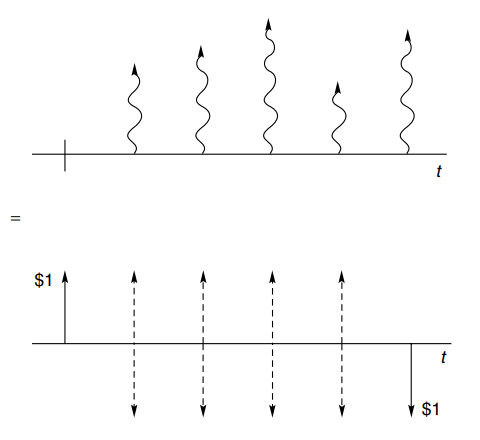
\includegraphics[width=0.65\linewidth]{Imagenes/Parte1/12_swaps/Interes_variable_swaps.png}
    \caption{Todos los intereses variables swap}
\end{figure}
Por lo tanto, el total de pagos por parte del interés variable es
\[
    1 - Z(t;T_N)
\]
siendo $Z(t;T_N)$ el valor actualizado de un bono de cupón cero y principal 1 (que es lo mismo que actualizar 1\$). 

Luego sumando el total de pagos de la parte del inetrés fijo y restando la parte del interés variable, el contrato swap para la parte variable es de:
\[
    r_s\tau \sum_{i=1}^N Z(t;T_i) - (1 - Z(t;T_N)) = \boxed{r_s\tau \sum_{i=1}^N Z(t;T_i) - 1 + Z(t;T_N)}
\]
para que el contrato tenga valor cero, el interés fijo debe ser debe
\begin{align}\label{eq:int_var}
    r_s\tau \sum_{i=1}^N Z(t;T_i) - 1 + Z(t;T_N) = 0 \Rightarrow \boxed{r_s = \frac{1 - Z(t;T_N)}{\tau \sum_{i=1}^N Z(t;T_i)}}
\end{align}
En vez de cero también se le puede dar cualquier valor.




\subsection{Bootstrapping}
El resultado anterior se puede usar para hacer el bootstrapping descrito en la sección~\ref{sec:forward_bootstrapping} para conseguir el valor de cupones cupón cero. Usando la ecuación~\eqref{eq:int_var}, se obtiene el valor de un bono de cupón cero y vencimiento $T_i$
\[
    r_s(T_1) = \frac{1 - Z(t;T_1)}{\tau Z(t;T_1)} \Rightarrow \boxed{Z(t;T_1) = \frac{1}{1+r_s(T_1)\tau}}
\]
y luego de forma iterativa
\[
    \boxed{Z(t; T_{j+1}) = \frac{1 - r_s(T_{j+1})\tau \sum_{i=1}^{j} Z(t; T_i)}{1 + r_s(T_{j+1})\tau}}
\]







\subsection{Otras características de contratos swap}
\begin{itemize}
    \item \textbf{Swaps Callable y puttable}: Permiten a un lado cerrar el contrato antes de vencimiento. Matemáticamente son del tipo opciones americanas, que se verán más adelante. 
    \item \textbf{Extendible swaps}: se puede ampliar el vencimiento con la tasa swap original.
    \item \textbf{Index amortizing rate swaps}: mientras que en los swaps vainilla el principal es constante (aunque nunca se llegue a pagar), en estos swaps el principal cambia con el tiempo siguiendo un calendario y muchas veces ligado a algún índice.
\end{itemize}





\subsection{Otros tipos de swaps}
\begin{itemize}
    \item \textbf{Basis Rate Swap}: los intereses son ambos variables ligados a distintos índices. P.e.\ un banco saca swaps de LIBOR contra los intereses que dan en los préstamos (que normalmente van ligados) para reducir riesgos en caso que dejen estar correlacionados.
    \item \textbf{Equity Swaps}: una parte paga interés fijo o flotante y la otra paga el retorno total de un índice bursátil (como el S\&P 500, EuroStoxx, etc.) incluyendo dividendos.
    \item \textbf{Equity basis swap}: como el anterior pero con dos índices distintos.
    \item \textbf{Currency Swaps}: dos partes intercambian flujos de efectivo en distintas divisas. P.e.\ una parte paga 1000\$ y la otra 1000\euro\ a un tipo de cambio preestablecido. Normalmente se intercambia el principal al inicio y al final del contrato.
\end{itemize}







